\documentclass{article}
\usepackage[utf8]{inputenc}
\usepackage{parskip}
\usepackage{mathrsfs}
\usepackage{graphicx}
\graphicspath{ {./images/} }

\title{Estimating wine quality with different sampling method}
\date{November 2020}

\begin{document}

\maketitle
\noindent NAME: Zongyang Gao\hfill Student Number: 95244521\par
Role and contributions: Data collection and data summaries, Data analysis, conclusion and discussion, article organization
\newline 

\noindent NAME: Yiqi Xu\hfill Student Number: 48148571\par
Role and contributions: Data analysis, conclusion and discussion
\newline 

\noindent NAME: Qiming Chen\hfill Student Number: 91723338\par
Role and contributions: Introduction\newline 

\noindent NAME: Catherine Cai\hfill Student Number: 52204310\par
Role and contributions: Data analysis\newline 
\newpage
\section{Introduction}
\paragraph{} 
Started from many thousands of years ago, humans from different countries produced and consumed wine with different customs. In contemporary society, the wine becomes much popular and a consumable drink for a wider range of people. With a large amount of wine consumption, it comes with a higher demand for appreciating high-quality wine. As Schnabel and Storchmann (2010) point out in their research, the information of wine quality is usually not transparent to the consumers, which leads to a high price signal set up by the high-quality producers to inform the consumers about their high standard but also comes with a high price set by the low-quality producers utilizing the asymmetric information.[1] Hence, an investigation of wine quality is crucial for disclosure of the hidden wine industrial information to form a healthier and more efficient market.
\paragraph{}
As one of the top ten wine exporting countries, Portugal contributed to the wine industry with 3\% of the market share in 2019 [3]. However, the name of Portuguese wine remains unfamiliar outside of Portugal and the study of Portuguese wine is insufficient. In this research, we aim to investigate the average quality and the high-quality ratio of Portuguese wine based on analytical data. This study will sample both red and white variants of the Portuguese "Vinho Verde" wine from the available dataset provided by UC Irvine Machine Learning Repository with a random sampling method and a stratified method based on the wine type.
\paragraph{}
Though the difficulty of studying wine is high due to the lack of an official or unified mainstream evaluation system for wine quality, a widely acknowledged wine-scoring scale was publicized by Robert Parker in his Wine Advocate newsletter and by Wine Spectator magazine [4]. The 100-point wine-scoring system scales at a range from 50 (unrecommended) to 100 (classic), which provides a straightforward and simple rubric to follow. The inconsistency of wine quality assessments can also serve as uncertainty to our quantitative analysis. The researchers recommend using teams of tasters, rather than sole taster, to work on the evaluation grading can reduce the inconsistency of wine quality assessments. [2] Despite the wine quality in the sample dataset of our study was evaluated and quantified by a professional group made of at least three sensory assessors using a blind test to avoid inconsistency, the grading scale is ranging from 0 to 10. Thus, we will convert the acknowledged 50 to 100 wine-scoring scale into the 0 to 10 grading scale for analyzing the high-quality ratio of wine in further sections.
\paragraph{}
With the analysis of the wine quality of Portuguese wine, our paper will benefit the consumers by providing information on the overall wine quality as an indicator of wine purchase. It can also be an indicator of high-quality sellers to adjust the price signal for their products. The analysis results in this study can be used in future studies to further explore the correlation between price and quality to examine the asymmetric information of the Portuguese wine market. 
\section{Data collection and data summaries}
\subsection{Overall Wine Data}
\paragraph{}
This study will consider \textit{vinho verde}, a unique product from Mineo (NW) in Portugal.It accounts for 15\% of Portugal's total wine production, mainly white.In this work, we will analyze the two most common varieties, white and red, from the \textit{vinho verde} demarcated area.Data were collected from May 2004 to February 2007, using only samples of protected origin tested in official certified Entity (CVRVV).[1]
\paragraph{}
In this study, the mean value of wine quality was the parameter of interest.As for preferences, each sample was assessed by at least three sensory reviewers (using blind tasting), who rated the wine on a scale of 0 (poor) to 10 (excellent).[1]
\subsection{Sampling Method}
\paragraph{}
In this study, two data sets are established, among which 1599 samples are red and 4898 samples are white.During the pre-processing phase, the database is transformed so that each row contains a different wine sample (including all tests). The final sensory score was given by the median of these evaluations.A histogram Figure \ref{figure:1} of the target variable is plotted to represent a typical normal distribution.[1]
\begin{figure}[h]
    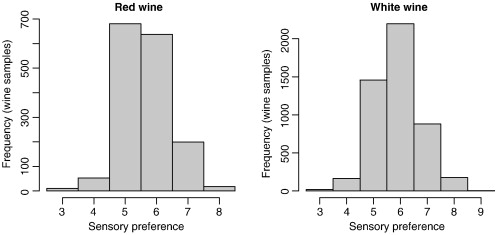
\includegraphics[width=\textwidth]{1.jpg}
    \caption{The histograms for the red and white sensory preferences}
    \label{figure:1}
\end{figure}
\paragraph{}
Two sampling methods are conducted in this study, SRS (simple random sample) and stratified sample. The targeted population is 6497 wines (1599 red and 4898 white). A sample with sample size 50 ($ n = 50 $) is randomly selected and a stratified sample with two strata is selected. When considering stratified sample, the sample is stratified by Red/White (i.e. the types of wines). Because the red and white tastes are quite different, the analysis will be performed separately. Since this study only consider the quality of wines, the result is still conclusive. When introducing more variables, it is suggested that the analysis is better to be performed separately.
\paragraph{}
This research will estimate two parameters. The first parameter is the average score of wines (numeric), it reflects the quality of wines in \textit{vinho verde}. The other parameter is the excellence rate, which refers the high-quality ratio of wines (binary). In this study, we convert the acknowledged 50 to 100 wine-scoring scale into the 0 to 10 grading scale and record wines with a score equal or above 7 as a quality wine. 
\section{Data Analysis}
\subsection{Simple random sampling}
\paragraph{}
We first start by taking simple random sample from both red and white wine. We take 50 samples from 6497 wines, and for these 50 samples, we get an estimate of average quality of wines, which is $\hat{y}=5.86$, with the standard error of $se(\hat{y})=\sqrt{{(1-\frac{n}{N})}\frac{var({y}_{s})}{n}}=0.1138807$, and 95\% confidence interval (5.720109 6.119891). 
\paragraph{}
In the second stage, we explore the high-quality ratio of wines, which is the proportion of wines with a score of quality equal or above 7. From these 50 sample, we observed 11 out of 50 with quality score equal or higher than 7. The estimate of the high-quality ratio is then  $\hat{\mu}=0.22$, with standard error $se(\hat{\mu})=\sqrt{{(1-\frac{n}{N})}\frac{\hat{\mu}(1-\hat{\mu})}{n}}=0.05835741$, and a 95\% confidence interval (0.1056195, 0.3343805).
\paragraph{}
In conclusion of SRS, we can see that the average quality of wines is 5.86 and the high-quality ratio is 0.22.
\subsection{Stratified sampling}
\paragraph{}
For another sampling method, we choose stratified sampling. We see that the ratio of the number of red wines to white wine is 1599:4898 = 1:3.063. According to this ratio, we now randomly select 12 wines from red wines and randomly selected 38 wines from white wines, and calculate estimates.
\paragraph{}
For these 50 samples, we get an estimate of average quality of wines  $\hat{y}_{str}=5.698391$, with the standard error of $se(\hat{y}_{str})=\sqrt{\sum_{h=1}^{H}({\frac{{N}_{h}}{N}})^2(1-\frac{{n}_{h}}{{N}_{h}})\frac{{s}^{2}_{{S}_{h}}}{n}}=0.09015076$, and 95\% confidence interval (5.521696, 5.875087).
\paragraph{}
For the high-quality ratio of wines, from these 50 sample, we observed 0 out of 12 red wines and 6 out of 38 white wines with quality score equal or higher than 7. The estimate of the high-quality ratio is then $\hat{\mu}_{str}=0.1190347$, with standard error $se(\hat{\mu}_{str})=\sqrt{\sum_{h=1}^{H}({\frac{{N}_{h}}{N}})^2(1-\frac{{n}_{h}}{{N}_{h}})\frac{\hat{\mu}_{str}(1-\hat{\mu}_{str})}{n}}=0.03872547$ , and a 95\% confidence interval (0.04313278, 0.19493661).
In conclusion of SRS, we can see that the average quality of wines is 5.698391 and the high-quality ratio is 0.1190347.
\subsection{Discussion}
\paragraph{}
Through previous data analysis, we can see that the average quality of wines estimated by SRS and stratified sampling is almost same. Consider the standard error of these two estimates, the standard error of estimated of the stratified sample is smaller than SRS. When consider the high-quality ratio, the ratio estimated by two methods is different and the standard error of stratified sample is smaller. Hence the advantage of stratified sample is when the internal stratification of a population is obvious, stratified sampling can improve the representativeness of the sample, so as to improve the accuracy of population inference from the answer sample, and disadvantage of stratified sampling is the sampling procedure is more complicated than random sampling, which also needs more information to make proper strata. For further consideration, when the overall sample size is small, some strata sample size is too small to be representative. SRS is most common method used in statistical learning, it has simple sampling procedure and easy to conduct. However, the result of SRS is not so precise since it used less information.

\section{Conclusion and Discussion}
\paragraph{}
In conclusion, the average quality of wines is 5.86 and the high-quality ratio is 0.22 (SRS). When the sample size is small, the strata sample might not be representative if the related strata sample size is too small. The result can be generalized to larger population.
\section{Appendix}
\paragraph{}
The link of the dataset is http://archive.ics.uci.edu/ml/datasets/Wine+Quality.
\paragraph{}
The code used is below:
\begin{figure}[h]
    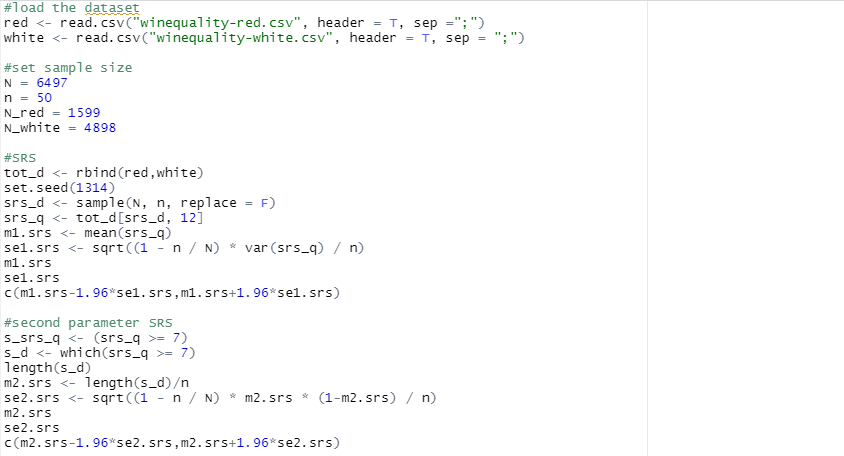
\includegraphics[width=\textwidth]{2.png}
    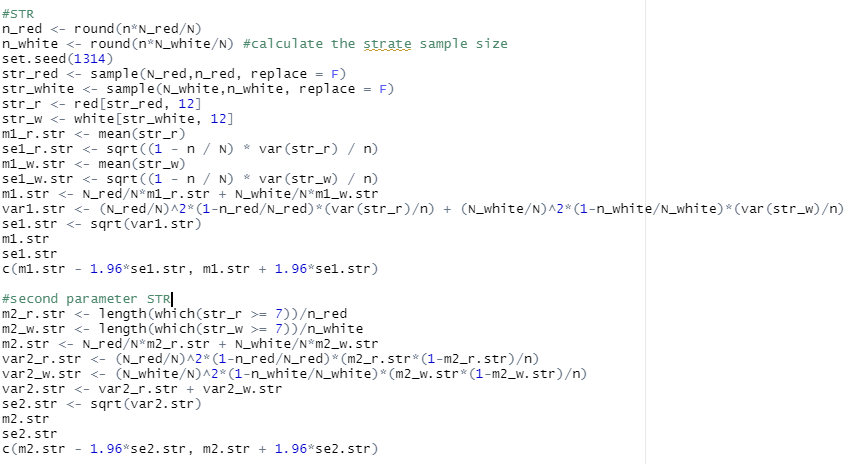
\includegraphics[width=\textwidth]{3.png}
\end{figure}

\newpage
\begin{thebibliography}{9}
\bibitem{Cortez} 
Cortez, P., Cerdeira, A., Almeida, F., Mato, T., Reis, T. (2009) Modeling wine preferences by data mining from physicochemical properties. 
\textit{Decision Support Systems}, 47(4), 547-553.

\bibitem{Oczkowski} 
Oczkowski, E., Doucouliagos, H. (2014) Wine Prices and Quality Ratings: A Meta‐regression Analysis.
\textit{American Journal of Agricultural Economics}, 97(1), 103-121.

\bibitem{Top25} 
Top 25 Wine Export Countries. (2019, March 15). Retrieved November 12, 2020, from https://www.reinisfischer.com/top-25-wine-export-countries

\bibitem{WineScores} 
What are Wine Scores? (n.d.). Retrieved November 12, 2020, from https://www.wine-searcher.com/wine-scores


\end{thebibliography}

\end{document}
